This layer is the integration of the UI and camera in details.

\begin{figure}[h!]
	\centering
 	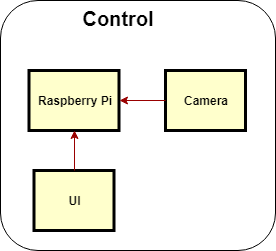
\includegraphics[width=0.60\textwidth]{images/Control_Layer}
 \caption{Control layer diagram}
\end{figure}

\subsection{User Interface}
The user interface operate through a browser that allow the user to give specifics task to the UR5.

\subsubsection{Assumptions}
The browser the user will be using is google chrome. Other browser may works just as well, this project however, has been operating the UI through google chrome.

\subsubsection{Responsibilities}
The purpose of this UI is to allow the user to gives specific command to the UR5. The commands are as follow::
	Home  		: Move UR5 to default position.
	Start 		: Make grill cheese sandwich.
	Stop  		: Cease function.
	Rack Tool 	: Put away tool.
	Grab Tool 	: Grab tool.
	
*The tools for this project specifically is a spatula. Other tools will be implement later in the future.

\subsubsection{Subsystem Interfaces}
The UI connects to the raspberry pi.

\begin {table}[H]
\caption {UI interfaces} 
\begin{center}
    \begin{tabular}{ | p{1cm} | p{6cm} | p{3cm} | p{3cm} |}
    \hline
    ID & Description & Inputs & Outputs \\ \hline
    \#xx & Rasberry Pi & \pbox{3cm}{N/A} & \pbox{3cm}{UI \\ Commands}  \\ \hline
    \end{tabular}
\end{center}
\end{table}

\subsection{Camera}
The camera use to determine the location of certain object(sandwich) or if there is another object in the way of the UR5.

\subsubsection{Assumptions}
The camera is a 720p or higher.
At least one camera.

\subsubsection{Responsibilities}
The purpose of the camera is to determine the location of the sandwich relative to its position so that the UR5 can pick up the sandwich. Its other responsibility is also to detect foreign obstacle or human being so that it can stop before colliding.

\subsubsection{Subsystem Interfaces}
The camera connects to the raspberry pi.

\begin {table}[H]
\caption {Camera interfaces} 
\begin{center}
    \begin{tabular}{ | p{1cm} | p{6cm} | p{3cm} | p{3cm} |}
    \hline
    ID & Description & Inputs & Outputs \\ \hline
    \#xx & Rasberry Pi & \pbox{3cm}{N/A} & \pbox{3cm}{Location of sandwich\\ Detect foreign obstacle or human being}  \\ \hline
    \end{tabular}
\end{center}
\end{table}

\subsection{Raspberry Pi}

\subsubsection{Assumptions}

\subsubsection{Responsibilities}

\subsubsection{Subsystem Interfaces}

\begin {table}[H]
\caption {Raspberry Pi interfaces} 
\begin{center}
    \begin{tabular}{ | p{1cm} | p{6cm} | p{3cm} | p{3cm} |}
    \hline
    ID & Description & Inputs & Outputs \\ \hline
    \#xx & UI & \pbox{3cm}{N/A} & \pbox{3cm}{N/A}  \\ \hline
    \#xx & Camera & \pbox{3cm}{N/A} & \pbox{3cm}{N/A}  \\ \hline
    \end{tabular}
\end{center}
\end{table}

